\documentclass[conference]{IEEEtran}

%XXX Remove before final submission
\usepackage{todonotes}
\usepackage{cite}
\usepackage{amsmath}
\usepackage{caption}
\usepackage{subcaption}
% Note that the amsmath package sets \interdisplaylinepenalty to 10000
% thus preventing page breaks from occurring within multiline equations. Use:
%\interdisplaylinepenalty=2500
% after loading amsmath to restore such page breaks as IEEEtran.cls normally
\usepackage{url}
\usepackage{hyperref}
\usepackage{verbatim}
\usepackage{siunitx}
\usepackage{listings}

\lstdefinelanguage{Julia}{
  basicstyle=\small\ttfamily,
  showspaces=false,
  showstringspaces=false,
  keywordstyle={\textbf},
  morekeywords={if,else,elseif,while,for,begin,end,quote,try,catch,return,local,abstract,function,stagedfunction,macro,ccall,finally,typealias,break,continue,type,global,module,using,import,export,const,let,bitstype,do,in,baremodule,importall,immutable},
  escapeinside={~}{~},
  morecomment=[l]{\#},
%  commentstyle=\textsf,
  commentstyle={},
  morestring=[b]",
}

\lstset{language=Julia,basicstyle=\footnotesize\ttfamily,breaklines=true}

% correct bad hyphenation here
\hyphenation{}


\begin{document}

%XXX remove before submission
\newcommand{\TODO}[1]{\todo[inline]{#1}}
\newcommand{\TODOFIG}[1]{\missingfigure{#1}}

\title{Which Program Is Slower? Hypothesis Testing for Performance Regressions}

% author names and affiliations
% use a multiple column layout for up to three different
% affiliations
\author{\IEEEauthorblockN{Jiahao Chen and Jarrett Revels}
\IEEEauthorblockA{Computer Science and Artificial Intelligence Laboratory\\
Massachusetts Institute of Technology\\
Cambridge, Massachusetts 02139--4307\\
Email: \{jiahao,jrevels\}@csail.mit.edu}
}

% make the title area
\maketitle

%%%%%%%%%%%%%%%%%%%%%%%%%%%%%%%%%%%%%%%%%%%%%%%%%%%%%%%%%%%%%%%%%%%%%%%%%%%%%%%%%%%%%%%%%%%%
\begin{abstract}
We propose a rigorous methodology for automated microbenchmarking and regression detection
in the presence of timer error, OS jitter and other environmental fluctuations. By examining
data obtained from Julia microbenchmarks, we demonstrate the ways in which timing
distributions can violate many of the statistical assumptions made by other benchmarking
frameworks. From our experimental observations, we construct a model and an accompanying
microbenchmarking strategy which purposefully avoids these assumptions. This strategy makes
efficient use of user time constraints by simultaneously maximizing the number of
measurements per trial while minimizing inter-measurement timing variations, rendering it
suitable for continuous integration (CI) pipelines, even when applied to relatively large
benchmark suites. Using our model, we formulate a robust, nonparametric hypothesis test that
makes use of the bootstrap resampling method to estimate the statistical significance of
observed variations in execution time. We test our methodology on a small collection of mock
Julia benchmarks, discussing where it succeeds relative to other methods as well as pointing
out potential pitfalls. Finally, we discuss a prototype implementation of the proposed
method that was recently released to aid in the development of the Julia language and
ecosystem, which has already caught and prevented several performance regressions in Julia's
base library.
\end{abstract}

\IEEEpeerreviewmaketitle

\TODO{come up with better section/subsection names}

%%%%%%%%%%%%%%%%%%%%%%%%%%%%%%%%%%%%%%%%%%%%%%%%%%%%%%%%%%%%%%%%%%%%%%%%%%%%%%%%%%%%%%%%%%%%
\label{sec:intro}
\section{Introduction}

Developers of high performance applications often rely on microbenchmark suites to determine
the impact of code changes on program performance. Despite the importance of these suites in
safeguarding against performance regressions, developers often run and interpret them in an
ad-hoc manner. This lack of a rigorous microbenchmarking methodology is dangerous, at best
wasting developers' time and at worst encouraging misguided code alterations that damage
performance instead of improve it.

The purpose of this paper is to introduce the reader to the difficulties of designing and
implementing a microbenchmarking methodology, and to present a methodology that overcomes
these difficulties. Note that we only focus on \textit{microbenchmarks}, which we define as
benchmarks whose execution time is on or below the scale of microseconds (\num{1e-6}
seconds).

We should preface our discussion by stating the criteria we use to analyze existing
approaches. To emphasize the practical consequences of these criteria, we present them in
terms of the features that an ``ideal'' microbenchmarking framework might provide:

An ideal microbenchmarking methodology would \textit{produce reproducible measurements}
while \textit{respecting user time constraints}. It would \textit{automatically identify
regressions} between experimental trials, quantifying detection confidence using
\textit{rigorous estimates of statistical significance}. Wide adoption of the methodology
would require it to be \textit{portable}, functioning across all platforms relevant to the
application being benchmarked. In order to automatically prevent the introduction of new
regressions, the methodology must be \textit{suitable for inclusion in continuous
integration (CI) pipelines} alongside normal testing suites.

Unfortunately, there are signficant barriers to implementing these features in practice,
especially with regards to reproducibility. In the following section, we discuss how
existing approaches attempt to overcome these barriers, and argue that these approaches -
individually or combined - are not sufficient to meet our microbenchmarking criteria.

%%%%%%%%%%%%%%%%%%%%%%%%%%%%%%%%%%%%%%%%%%%%%%%%%%%%%%%%%%%%%%%%%%%%%%%%%%%%%%%%%%%%%%%%%%%%
\label{sec:challenges}
\section{Microbenchmarking is hard}

\subsection{Controlling for environmental effects is hard}

Modern hardware and operating systems present a large number of confounding factors that
complicate a developer's ability to reason about variations in user-space application
performance~\cite{HP5e}. These factors include...

\TODO{cite/elaborate on these where necessary}
\begin{itemize}
    \item ...changes in temperature, workload, and power availability that can trigger
    CPU frequency scaling.
    \item ...hardware and software interrupts which can disrupt timers and benchmark
    execution.
    \item ...kernel-controlled behaviors such as thread rescheduling, virtual addressing,
    and other quirks of memory configuration (paging, swapping, caching,
    etc.)~\cite{Oyama2014,Oyama2016}.
\end{itemize}

The literature refers to many of these factors - particular those triggered via the kernel -
as ``OS jitter''. Since timing variations due to OS jitter are difficult to distinguish from
timing variations due to genuine changes in application peformance, there is a wide corpus
of literature regarding OS jitter isolation and elimination. Research progress in this area
is highly platform-dependent, and mostly revolves around specialized kernel configurations,
compiler modifications, and VM tuning.

\TODO{discuss existing ``environmental'' research, see notes in comments}

\begin{comment}
Points to make:
    - VM research is probably skewed towards JVM
    - OS research is probably skewed towards Linux
Things to cite:
    - changing the heap size can affect garbage collector performance % cite - Blackburn et al. [4], Stephen M Blackburn, Perry Cheng, and Kathryn S McKin- ley. Myths and realities: The performance impact of garbage collection. In SIGMETRICS, pages 25–36. ACM Press, 2004.
    - OSs that provide a low-variability environment for program execution, such as NIX or Tesselation
    - tickless kernels featuring soft partitioning of cores and threads between application and systems processes~\cite{Akkan2012}.
    - replay compilation for reproducible binary layouts~\cite{Georges2008}
    - randomization of binary layouts to reduce correlation in timing measurements, in projects like to induce Gaussian timing distributions \textsc{Stabilizer}~\cite{Curtsinger2013}
        - (?) introduce nondeterminism in memory management
        - (?) determine the layout of binaries
    - paper citing thread scheduling problem in Linux
    - low-variability garbage collection in just-in-time compiler virtual machines~\cite{Huang2004}
    - strategies for orchestrating performance counters
    - Furthermore, seemingly irrelevant configuration parameters like the size of the UNIX
      environment can confound reproducibility. Changing the size of the environment moves the
      call stack, which is loaded after the environment, which in turn changes the alignment of
      data in memory~\cite{Mytkowicz2009}.
\end{comment}

In the end, microbenchmarking should not rely on system quiescence, since many techniques
for achieving quiescence are platform-dependent, require a high degree of deviation from
a user's personal OS/compiler configuration, or cannot be reasonably automated without
root access to the user's machine. Reliance on these techniques could negatively impact
portability and thus decrease the likelihood of adoption.

\subsection{Designing an experimental protocol is hard}

\TODO{cite/discuss Kalibera's paper on ``benchmarking in reasonable time'', and similar
papers}

\subsection{Doing stastistics on timing measurements is hard}
\begin{figure}
\centering
\begin{subfigure}{0.22\textwidth}
    \centering
    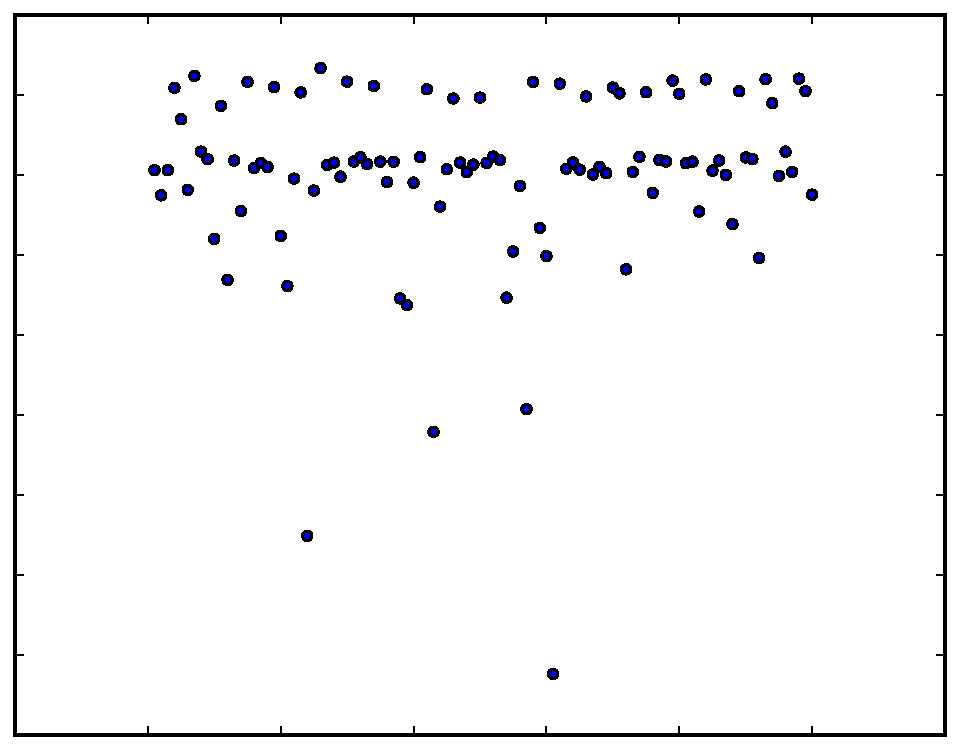
\includegraphics[width=\textwidth]{figures/fig1/simple_branchsum_fast}
    \caption{Benchmark 1: Unimodal}
\end{subfigure}%
~
\begin{subfigure}{0.22\textwidth}
    \centering
    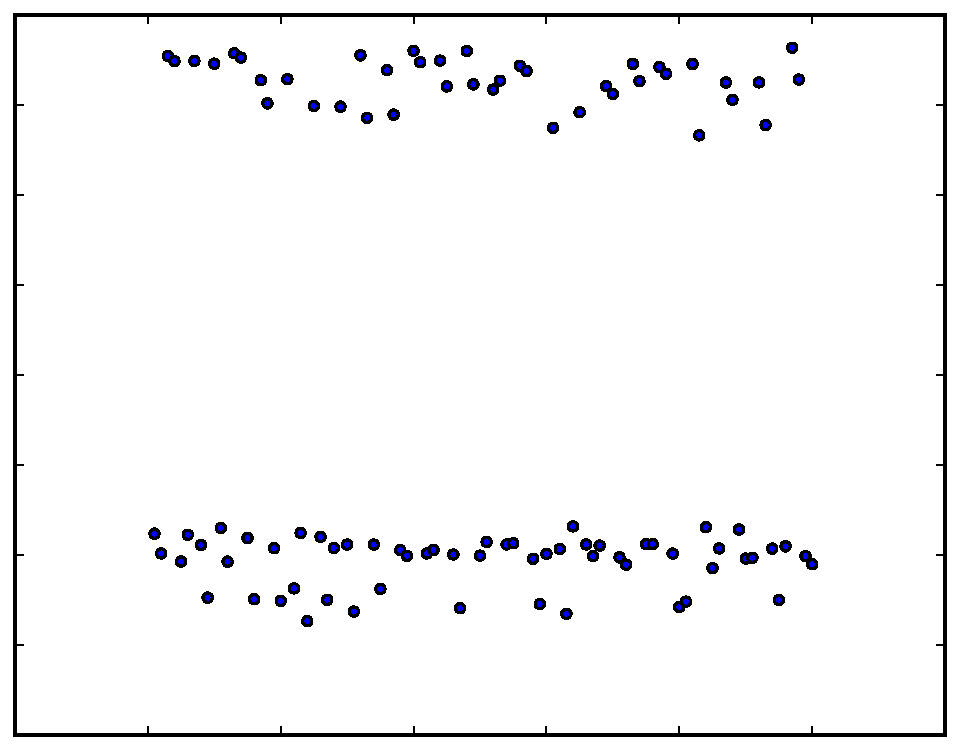
\includegraphics[width=\textwidth]{figures/fig1/bimodal_branchsum}
    \caption{Benchmark 2: Bimodal}
\end{subfigure}
\begin{subfigure}{0.22\textwidth}
    \centering
    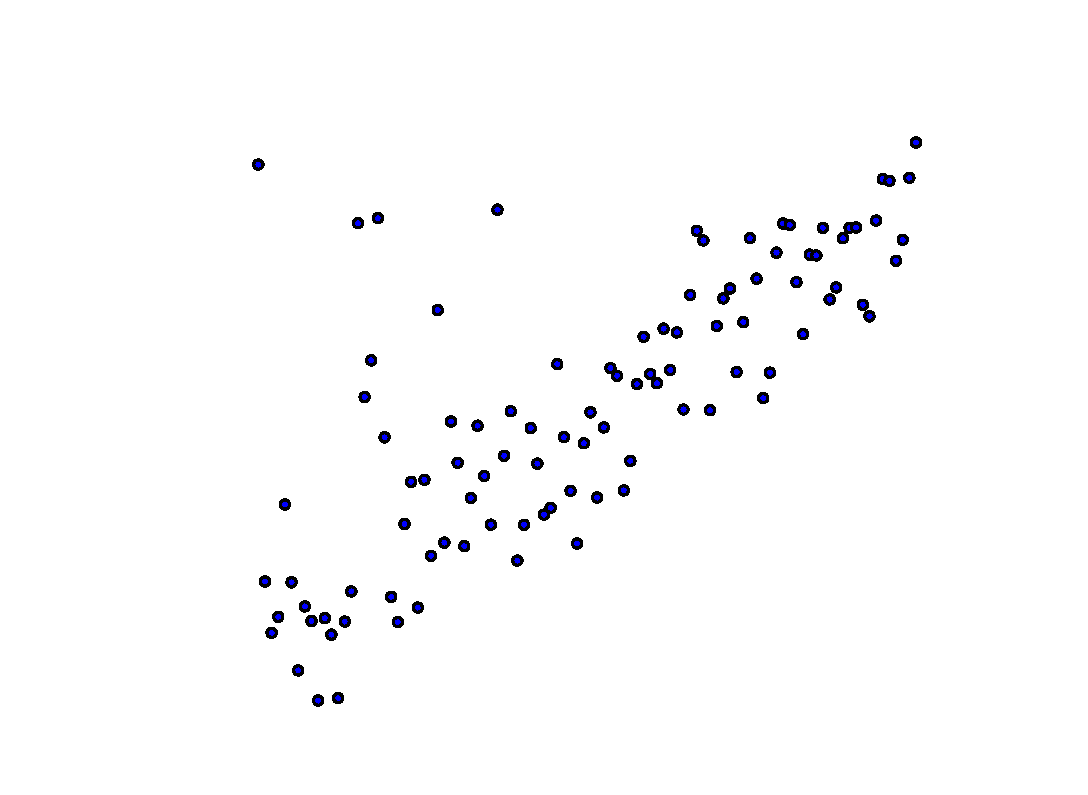
\includegraphics[width=\textwidth]{figures/fig1/drift_manyallocs_slow}
    \caption{Benchmark 3: Skewed}
\end{subfigure}
~
\begin{subfigure}{0.22\textwidth}
    \centering
    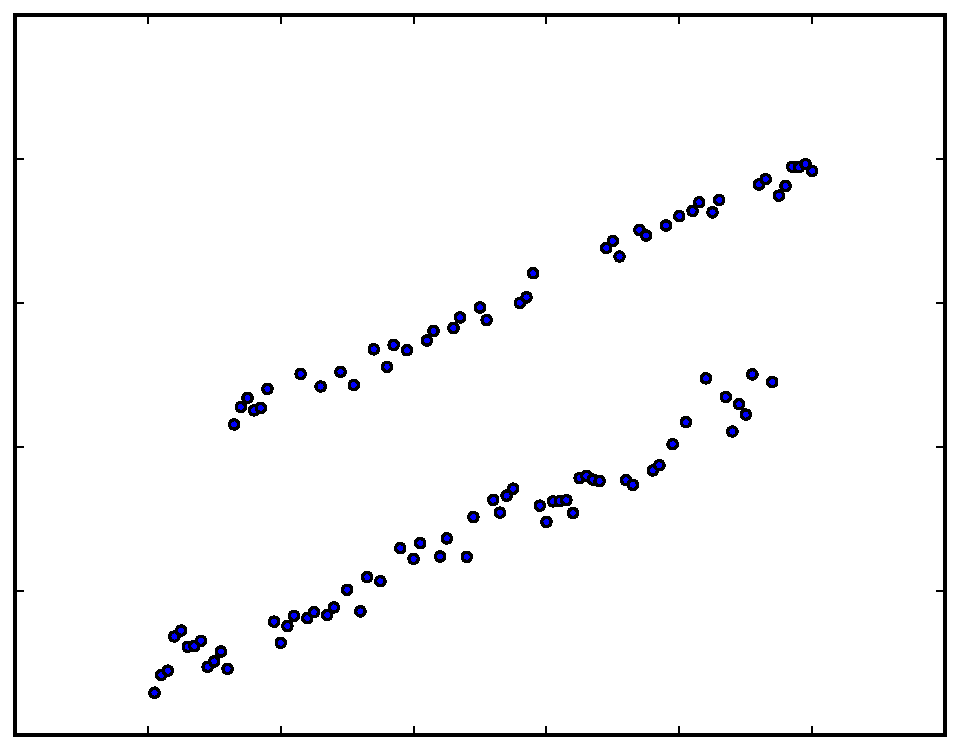
\includegraphics[width=\textwidth]{figures/fig1/bimodal_drift_sumindex}
    \caption{Benchmark 4: Bimodal + Skewed}
\end{subfigure}
\caption{Mean distributions for 4 different benchmarks. Each point is the mean time for a
         trial of 10,000 measurements. The x-axis is the index of the trial, while the
         y-axis is time.}
\label{fig:meandistributions}
\end{figure}

\TODO{cite/discuss papers that assume normality and/or that all benchmark timings are
identically distributed}

%%%%%%%%%%%%%%%%%%%%%%%%%%%%%%%%%%%%%%%%%%%%%%%%%%%%%%%%%%%%%%%%%%%%%%%%%%%%%%%%%%%%%%%%%%%%
\label{sec:stats}
\section{A better statistical interpretation of microbenchmark timing distributions}

%%%%%%%%%%%%%%%%%%%%%%%%%%%%%%%%%%%%%%%%%%%%%%%%%%%%%%%%%%%%%%%%%%%%%%%%%%%%%%%%%%%%%%%%%%%%
\label{sec:protocol}
\section{Experimental protocol for benchmark execution}

\begin{figure}
\centering
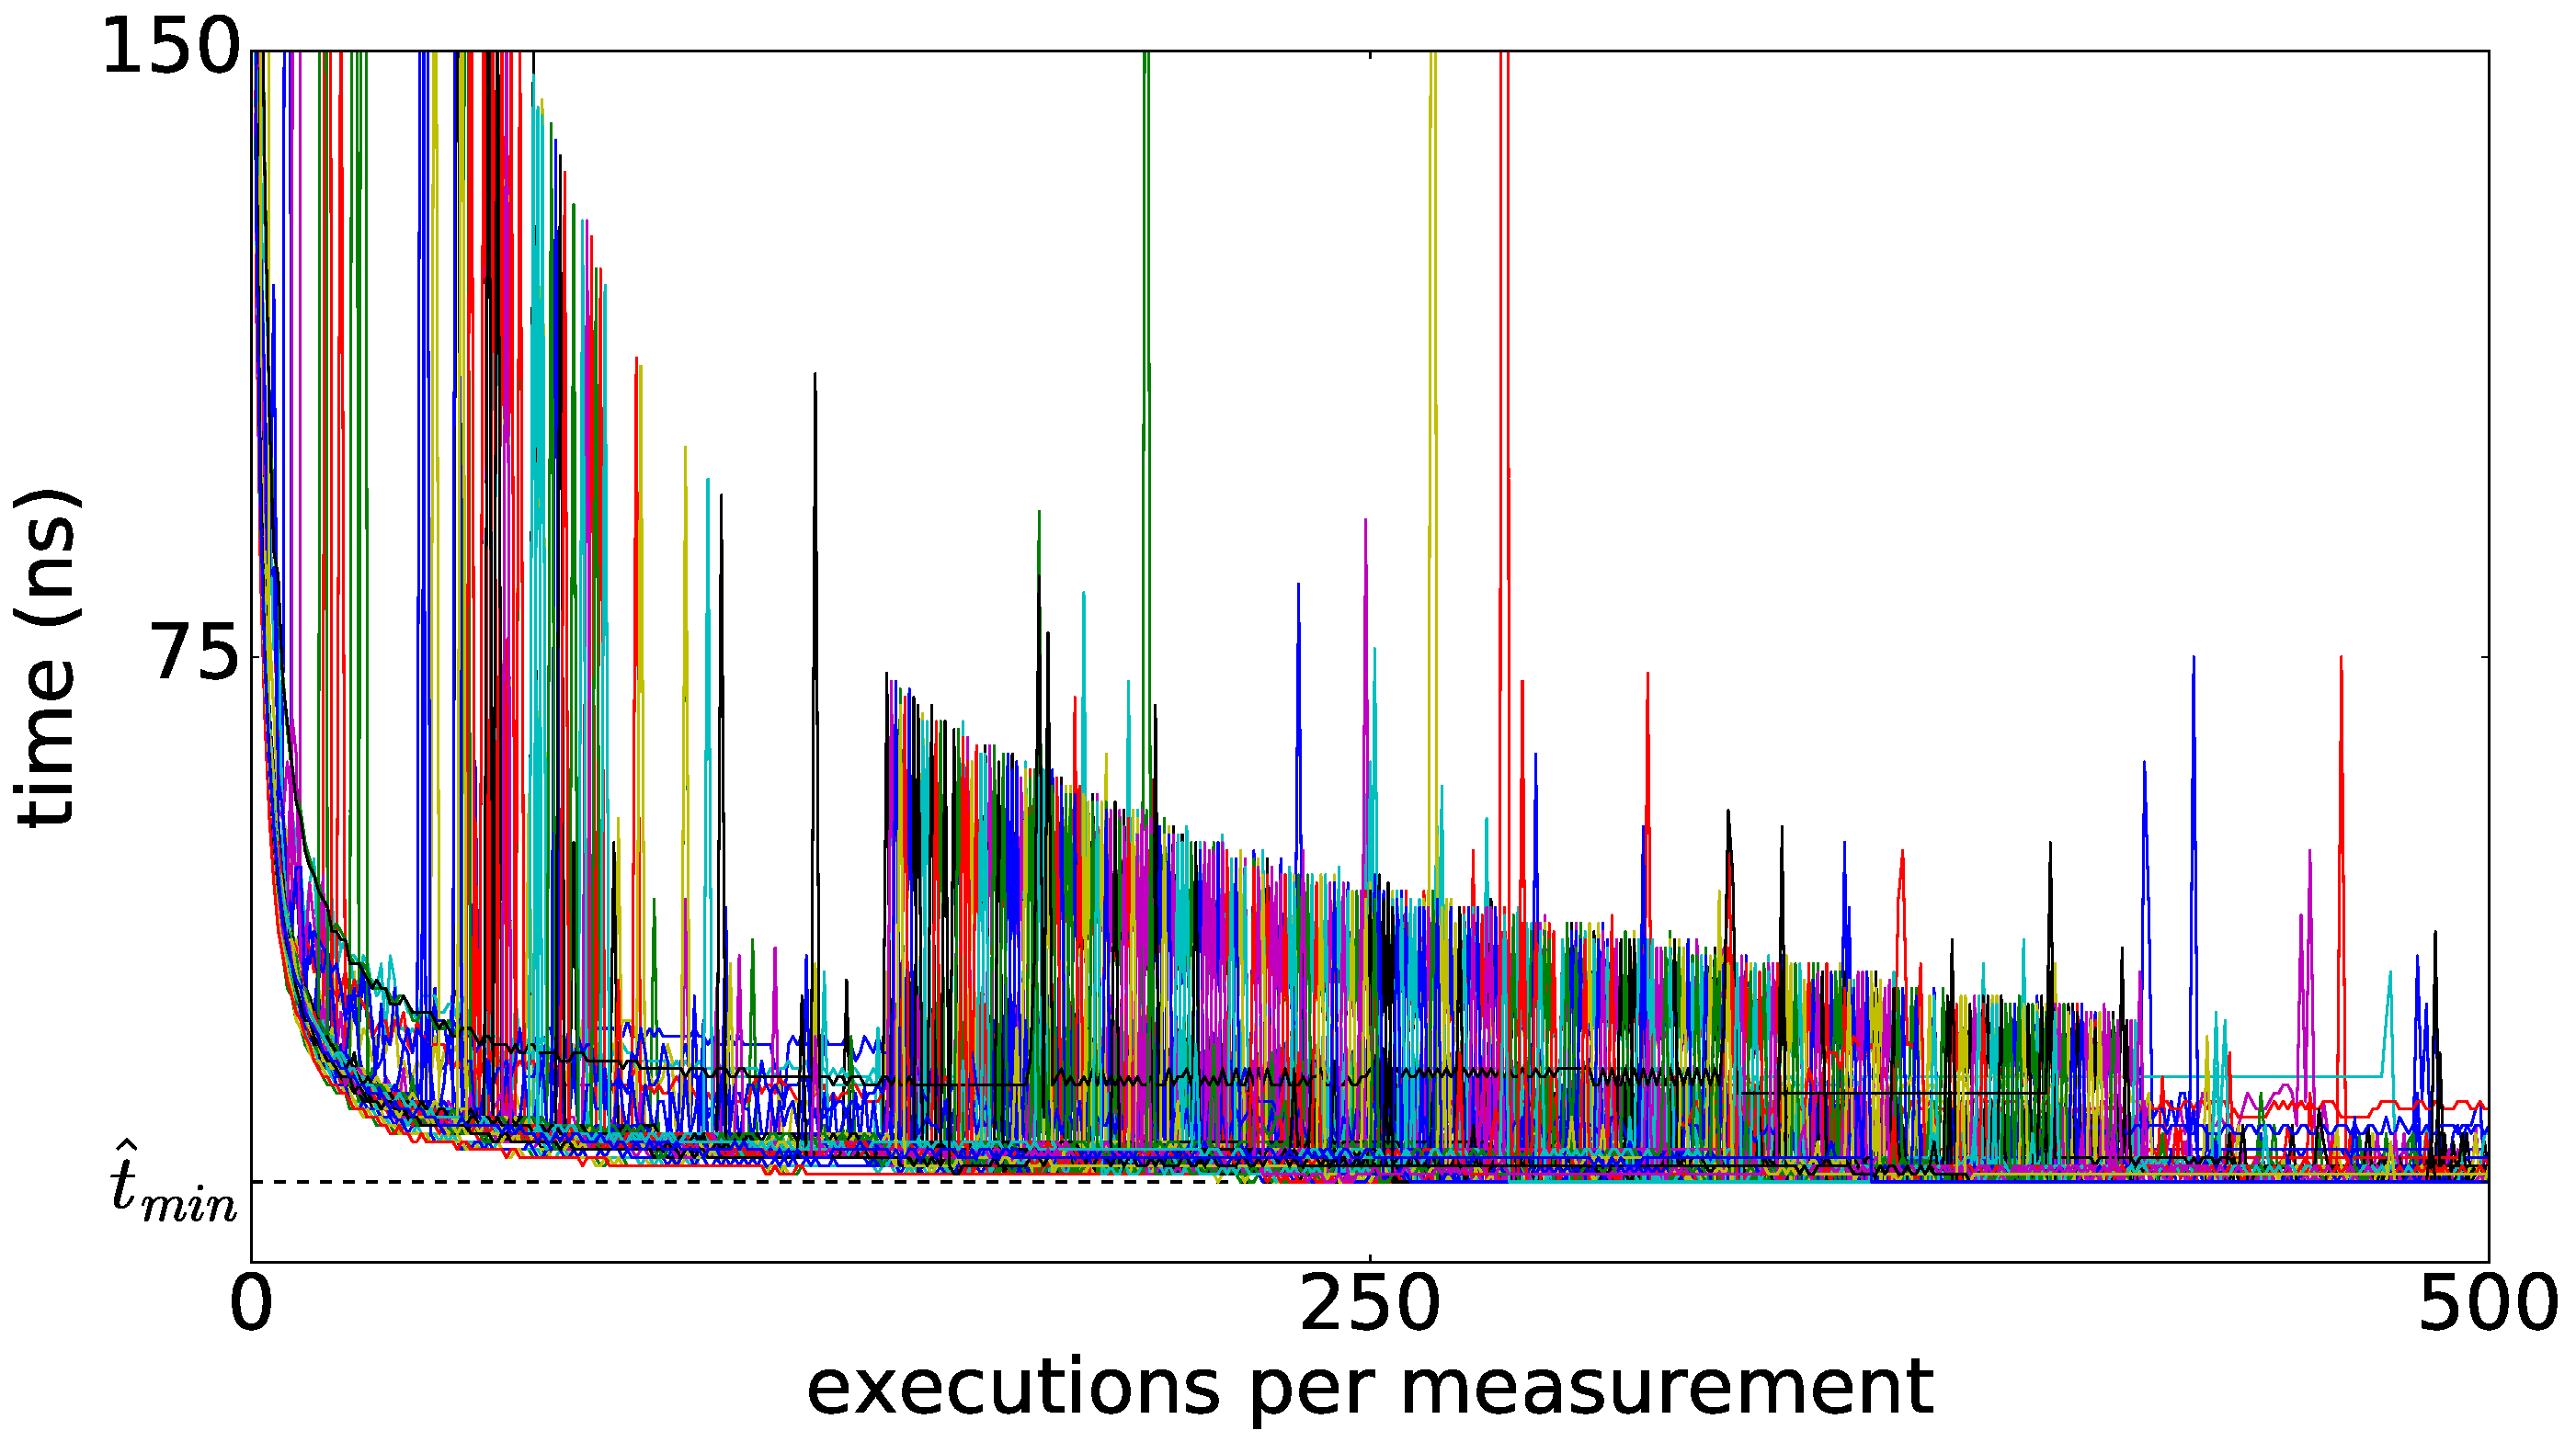
\includegraphics[width=0.45\textwidth]{figures/fig2/linear_scan_branchsum}
\caption{$t_j = T_j(n)/n$ for many repeated linear scans for a particular benchmark,
         where $T_j$ is defined in \eqref{eq:linsearch}. Each curve denotes a different
         linear scan. Note the large spikes produced by jitter.}
\label{fig:scaling}
\end{figure}

Given a benchmarkable program $P$ and a time budget $\tau_{budget}$, we'd like to define
$n$, the number of executions of $P$ to perform for each timing measurement, such that a
trial of our experiment...

\begin{itemize}
    \item ...produces timing estimates as close to the lower bound $t_{min}$ as possible
    \item ...minimizes the variance between timing estimates
    \item ...maximizes the number of timing measurements we are able to obtain under the
    constraint of $\tau_{budget}$
\end{itemize}

Given a timer accuracy $\tau_{acc}$ and a timer precision $\tau_{prec}$, our algorithm for
tuning $n$ is as follows:

\begin{enumerate}
    \item For $n \in \{1...\tau_{acc}\}$, measure the amount of time it takes to perform $n$
    executions of $P$. The result of this step is a collection of timing measurements $T_n$
    for all $n$.
    \item From the derived timing estimates $t_i = T_i / i$, select the minimum timing
    estimate $\hat{t}_{min}$.
    \item To obtain $n$, plug $\hat{t}_{min}$ into an oracle function $\nu(t_i) \to n_i$.
    Given $\tau_{acc}$ and $\tau_{prec}$, the properties of $\nu(t)$ are as follows:
    \begin{itemize}
        \item $\nu(\tau_{prec}) \approx \tau_{acc}$
        \item $\nu(\tau_{acc}) \approx \text{small} (\sim 10)$
        \item $\nu(t \gg \tau_{acc}) \approx 1$
        \item $\frac{d\nu}{dt}\big|_{t \approx \tau_{prec}} = \text{close to zero}$
        \item free of discontinuities \TODO{how to say this correctly since the range is
        discretized}
    \end{itemize}
\end{enumerate}

%%%%%%%%%%%%%%%%%%%%%%%%%%%%%%%%%%%%%%%%%%%%%%%%%%%%%%%%%%%%%%%%%%%%%%%%%%%%%%%%%%%%%%%%%%%%
\label{sec:hypotesting}
\section{Hypothesis tests for regression detection}

\begin{figure}
\centering
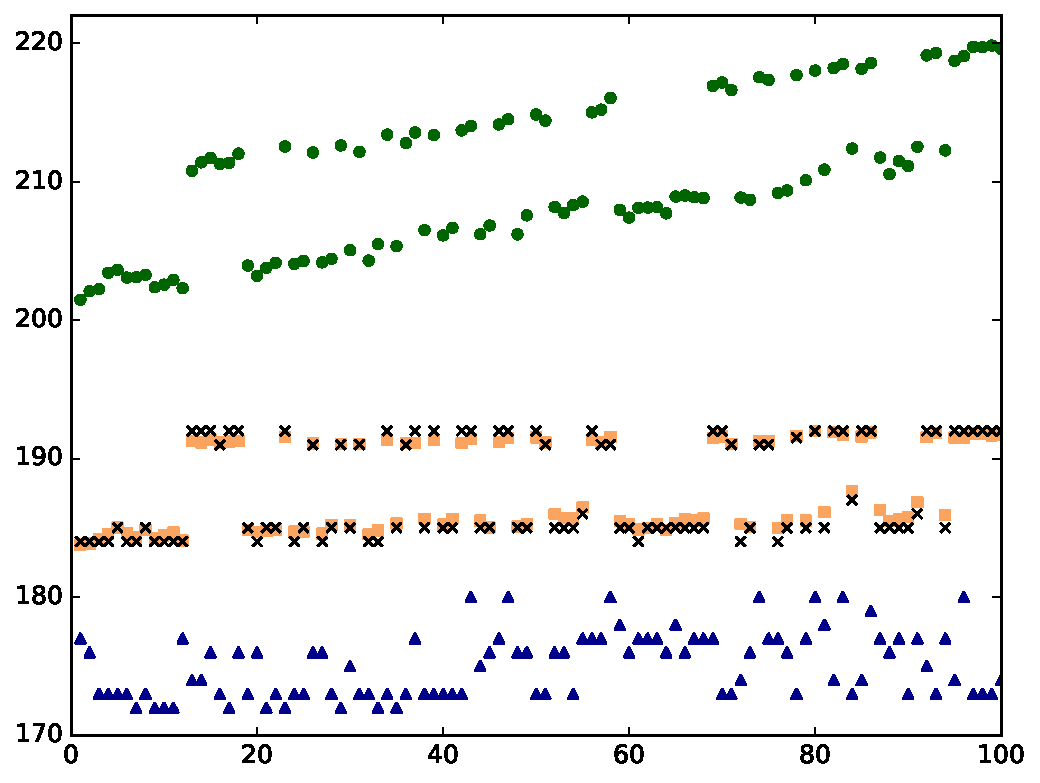
\includegraphics[width=\columnwidth]{figures/fig3/location_estimators_sumindex}
\caption{The behavior of different location parameters across multiple trials of
the \lstinline|sumindex| benchmark: mean (green filled circles), trimmed mean of
the 5th---95th percentiles (brown filled squares), medisn (black crosses), and
minimum (blue filled triangles).}
\label{fig:locationmeasures}
\end{figure}

%%%%%%%%%%%%%%%%%%%%%%%%%%%%%%%%%%%%%%%%%%%%%%%%%%%%%%%%%%%%%%%%%%%%%%%%%%%%%%%%%%%%%%%%%%%%
\label{sec:limits}
\section{Limitations of our methodology}

\begin{figure}[!t]
\centering
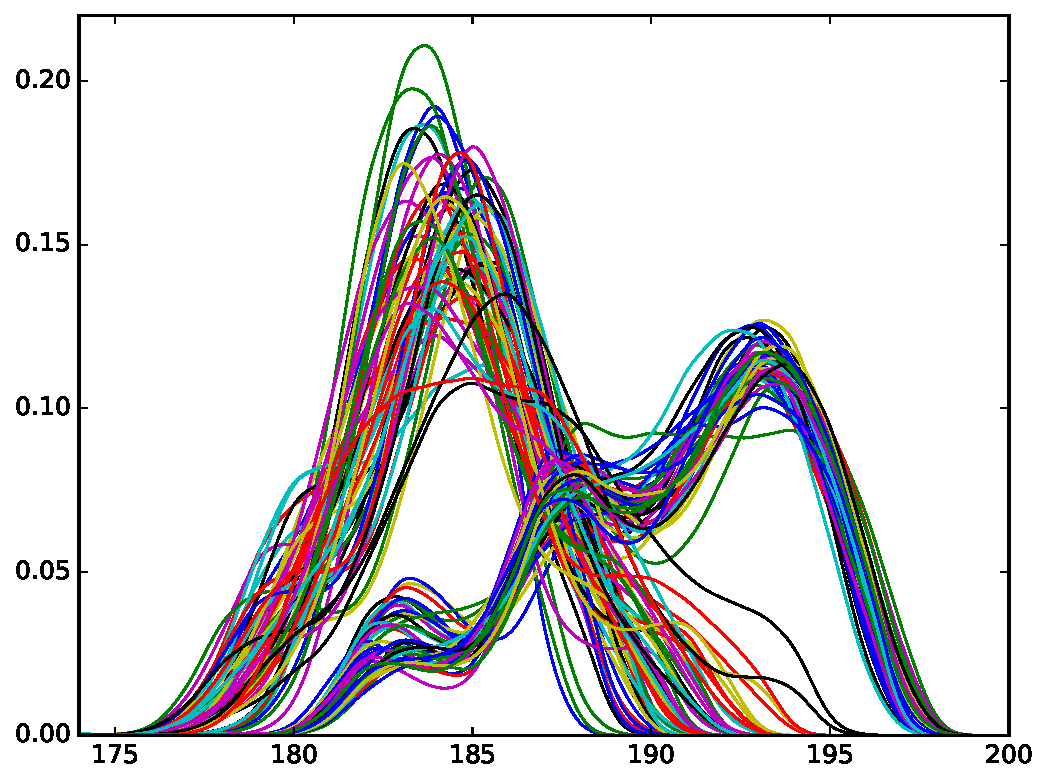
\includegraphics[width=\columnwidth]{figures/fig4/kde_pdf_sumindex}
\caption{Probability density functions (pdfs) from repeated trials of the
\lstinline|sumindex| benchmark. The pdfs form two distinct clusters, indicating
correlation across multiple trials.}
\label{fig:pdfsumindex}
\end{figure}

%%%%%%%%%%%%%%%%%%%%%%%%%%%%%%%%%%%%%%%%%%%%%%%%%%%%%%%%%%%%%%%%%%%%%%%%%%%%%%%%%%%%%%%%%%%%
\label{sec:julia}
\section{Implementation in Julia}

%%%%%%%%%%%%%%%%%%%%%%%%%%%%%%%%%%%%%%%%%%%%%%%%%%%%%%%%%%%%%%%%%%%%%%%%%%%%%%%%%%%%%%%%%%%%
\label{sec:conclusion}
\section{Conclusion}

%%%%%%%%%%%%%%%%%%%%%%%%%%%%%%%%%%%%%%%%%%%%%%%%%%%%%%%%%%%%%%%%%%%%%%%%%%%%%%%%%%%%%%%%%%%%
\label{sec:acknowledgement}
\section*{Acknowledgment}

We thank the many Julia developers, in particular Andreas Noack for many insightful
discussions. This work was supported by the Nanosoldier grant.\TODO{Get grant info}

%%%%%%%%%%%%%%%%%%%%%%%%%%%%%%%%%%%%%%%%%%%%%%%%%%%%%%%%%%%%%%%%%%%%%%%%%%%%%%%%%%%%%%%%%%%%
\bibliography{biblio}
\bibliographystyle{IEEEtran}

% that's all folks
\end{document}
\grid
